\chapter{GSAS-II Utility Computation Tools}\label{Chap:Utilities}

\section{Absorb: Compute X-ray Absorption Coefficient}\label{ref:Absorb}\index{program Absorb}

GSAS-II includes a program for computing the absorption of a material. It was originally created as a free-standing program that was also implemented as a web utility,
\footnote{A web calculator for x-ray absorption based on program Absorb is found at URL  https://11bm.xray.aps.anl.gov/absorb/}
but now is  accessed from inside the GSAS-II GUI. To access it, use the Calculate/"Run Absorb" menu command. This will open a window, as shown in Fig. \ref{fig:absorb1}. The next step in use is to add the elements that will be used in the computation. Use the Absorb/"New Element" menu command to add the elements that will be needed. After entering the menu command, a periodic table is shown, as seen in Fig. \ref{fig:absorb2}. Click on one or more elements in the table; note the color of the selected elements change as selected. Click on OK to close the periodic table window and return to the previous window for the Absorb program, which now lists computation results, but you will likely need to edit the chemical formula which is done by typing a number in the box to the right of the element and \textit{then pressing Enter}. 

\begin{figure}
    \centering
    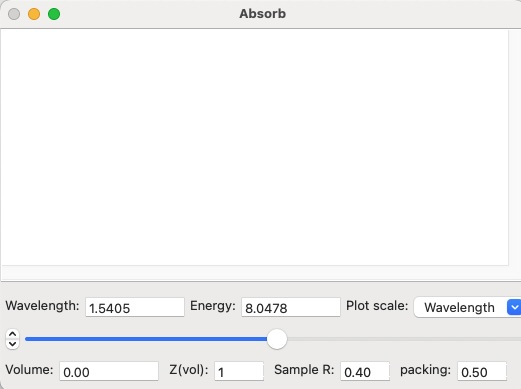
\includegraphics[width=0.5\linewidth]{figures/absorb1.jpg}
    \caption{Program Absorb: initial empty window}
    \label{fig:absorb1}
\end{figure}

\begin{figure}
    \centering
    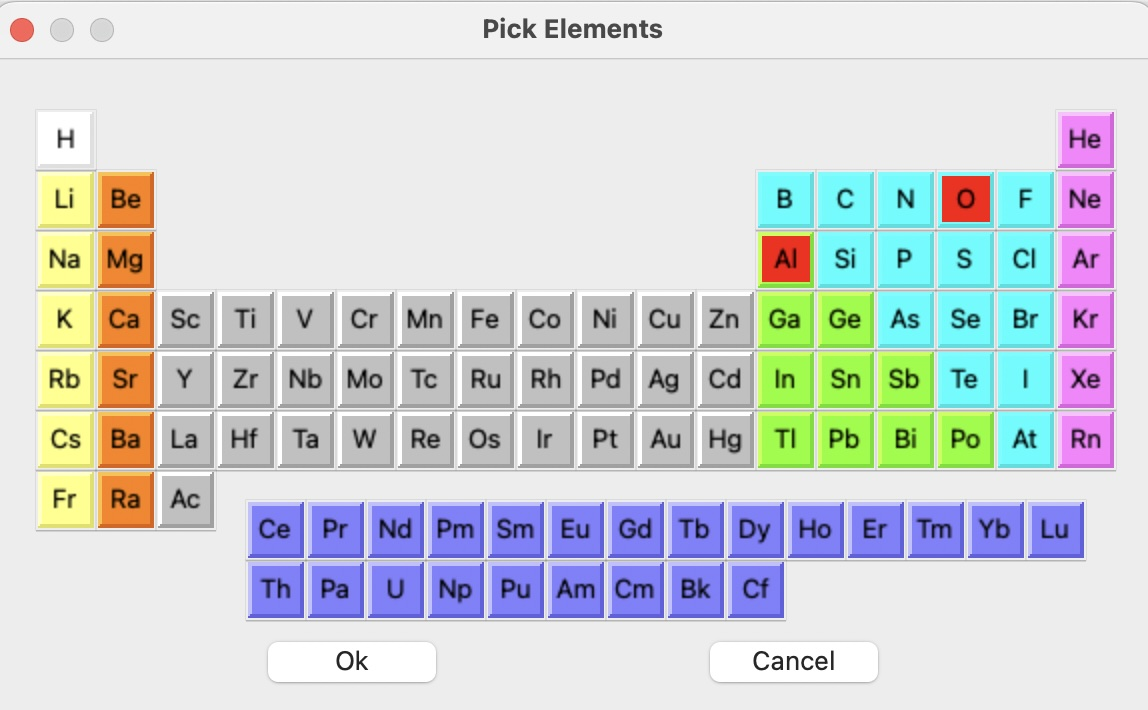
\includegraphics[width=0.5\linewidth]{figures/absorb2.jpg}
    \caption{Program Absorb: element selection}
    \label{fig:absorb2}
\end{figure}
Other input that you will likely supply includes the x-ray wavelength (or energy) and the sample radius (labeled as "Sample R") \textit{in mm}. Note that capillary dimensions are normally supplied as a diameter, so make sure you divide that by 2. The packing fraction (labeled here as "packing") is probably in the range of 0.4 to 0.6, so 0.5 is probably a good number. The "Volume" and "Z" values are used to estimate the crystallographic density, listed in the computations as the "Est. density". What is listed as the "powder density" is the crystallographic density multiplied by the packing fraction; this is the density used to compute x-ray absorption. The "Volume" and "Z" values likely do not need to be changed. Ideally, you will have measured the actual sample density, by weighing the sample and estimating the volume. If so, modify the packing fraction to get the powder density  to match what you measured. 

Note that the computations are not updated until you press "Enter" after changing any inputs. 
\begin{figure}
    \centering
    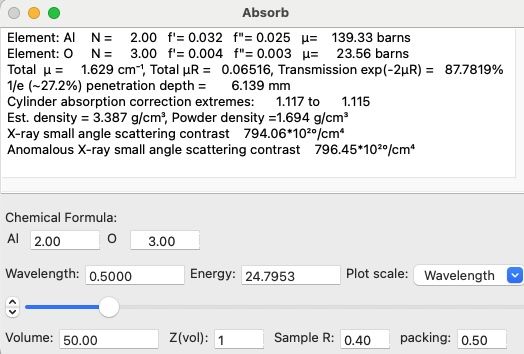
\includegraphics[width=0.5\linewidth]{figures/absorb3.jpg}
    \caption{Program Absorb: After element selection and stoichiometry editing}
    \label{fig:absorb3}
\end{figure}
The computed linear absorption coefficient value is reported as $\mu$ in cm${}^{-1}$, but for Debye-Scherrer geometry measurements, the key value is $\mu R$, as discussed in depth in section \ref{ref:muR}. Note the plots produced by program Absorb. The wavelength dependence plot will show if there are any absorption edges to be avoided and how much the wavelength will need to be changed to bring  $\mu R$ into the feasible range (red horizontal line) or recommended range (blue horizontal line). The correction vs. $2\theta$ plot shows how significant the correction will be over the data collection range. Note that this value is a measurement of transmission. A value of 20 indicates that only 95\% of the x-ray radiation is being lost to absorption. 

To confirm that a sample depth is thick enough for Bragg-Bretano measurements, you can also use program Absorb for that. Use the sample thickness divided by 2 as the radius. The transmission factor (listed after the $\mu R$ value) will represent the amount of x-ray radiation that would be transmitted through the sample at $2\theta$ of 180$^\circ$ and should be on the order of <5\% (noting that the path length increases by $1/cos\theta$ for $2\theta < 180^\circ$) as the actual losses will be lower.  

Use the Absorb/Quit menu command to exit the Absorb program. Exiting GSAS-II will also close Absorb.

\section{Fprime: Compute atomic scattering}\label{ref:Fprime}\index{program Fprime}

Resonant scattering (see section \ref{ref:resonantscattering}), also called anomolous dispersion, is in my opinion an underutilized technique in powder diffraction. Part of the reason for this is that these experiments are hard to perform, as it is usually quite difficult to make wavelength changes at  powder diffraction beamlines. This is not because wavelength changes are inherently difficult at synchrotrons. Spectroscopy beamlines routinely run scans of wavelengths. The difficulty is that no facility has designed an instrument that is dedicated to performing resonant scattering powder diffraction experiments. GSAS-II includes a program for computing the scattering factor curves for selected elements that is useful for planning resonant scattering measurements called Fprime. It is also useful for determining elements that would be problematic for a measurement at a particular x-ray wavelength. One always wants to avoid wavelengths that are slightly shorter than the edge, as this is where both absorption and fluorescence is most problematic.

Program Fprime. It uses the same computation method as GSAS-II does for estimation of $f^\prime$ and $f^{\prime\prime}$ values, which are taken from a compilation made in 1981 by D. T. Cromer\index{Cromer, D.} and D. A. Liberman.\index{Liberman, D.}. Note that these curves are approximate and the exact values will depend on the exact chemical environment of each atom. If the exact $f^\prime$ and $f^{\prime\prime}$ curves need to be known for some reason, one should perform a wavelength scan of absorption or fluorescence and then perform a Kramers-Kronig inversion, but resonant scattering experiments are typically performed 50-100 eV below the edge, where the $f^\prime$ and $f^{\prime\prime}$ values are not much affected by chemical shifts so the values from this program are accurate enough for these experiments. 

To access program Fprime, use the Calculate/"Run Fprime" menu command. This will open a window that is somewhat similar to the initial window in program Absorb (Fig. \ref{fig:absorb1}.) The next step in use is to designate the element(s) that will be used in the computation. Use the Fprime/"New Element" menu command to add the elements that will be needed. After entering the menu command, a periodic table is shown. This window is exactly the same as the periodic table used in Absorb, shown in Fig. \ref{fig:absorb2}. Click on one or more elements in the table; note the color of the selected elements change as selected. Click on OK to close the periodic table window and return to the previous window for the Fprime program, which now lists the selected elements and their $f^\prime$ and $f^{\prime\prime}$ values at the default wavelength, as seen in Fig. \ref{fig:fprime1}. The wavelength dependence of the $f^\prime$ and $f^{\prime\prime}$ values, as well as the form factors, are plotted in the graphics window, as shown in Fig. \ref{fig:fprime2}. Note that the plot x-axes can be changed from the main Fprime window. 

\begin{figure}
    \centering
    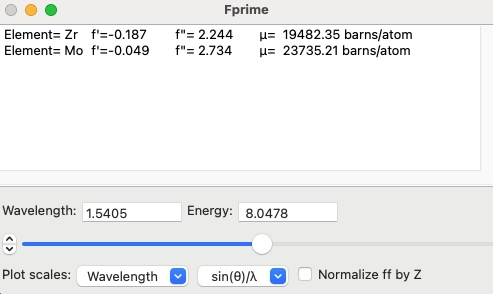
\includegraphics[width=0.5\linewidth]{figures/fprime1.jpg}
    \caption{Program Fprime: window after elements are added.}
    \label{fig:fprime1}
\end{figure}

\begin{figure}
    \centering
    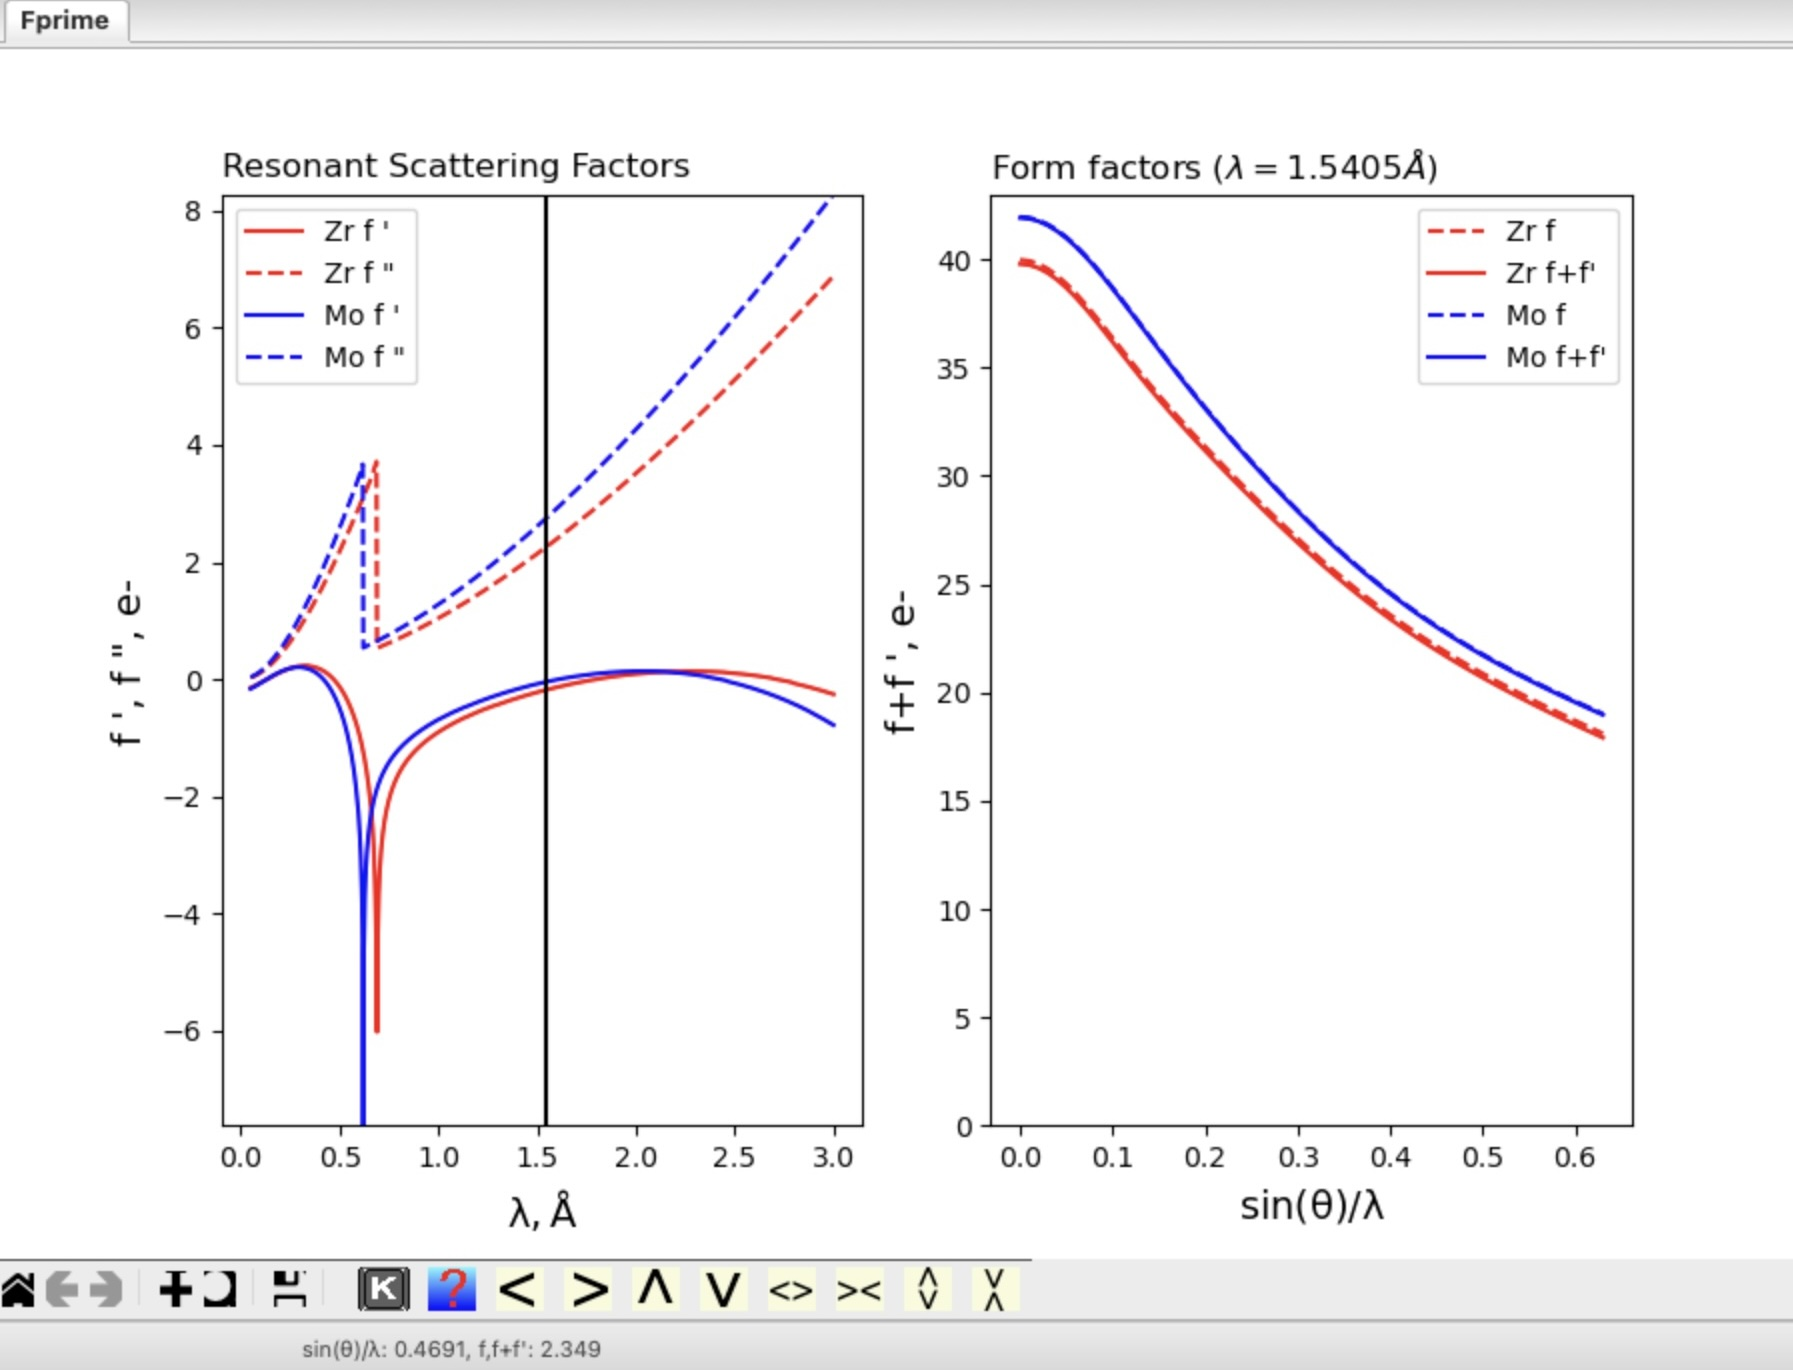
\includegraphics[width=1\linewidth]{figures/fprime2.jpg}
    \caption{Program Fprime: graphics window after elements are added.}
    \label{fig:fprime2}
\end{figure}

The wavelength/energy that is used to compute the $f^\prime$ and $f^{\prime\prime}$ values can be changed in several ways. On the main window, the slider can by dragged or a value can be typed into either box. Also, the value is shown as a black vertical line on the $f^\prime$ and $f^{\prime\prime}$ plot; this black line can be dragged. Fig. \ref{fig:fprime3} shows the change to the main window and  Fig. \ref{fig:fprime4} shows the change to the plot after the energy has been changed close to the Zr absorption edge. If the wavelength were just below (the energy just above) the Zr absorption edge, the $\mu$ value would be much higher. Note that due to the shift, relative to well away from the edge, the effective scattering power of Zr has been changed by a few electrons. This is not a large change, but the ability to measure both close to the edge and away from the edge would provide much greater sensitivity to Zr atom positions, if both datasets are used in a single refinement. 
   
    \begin{figure}
    \centering
    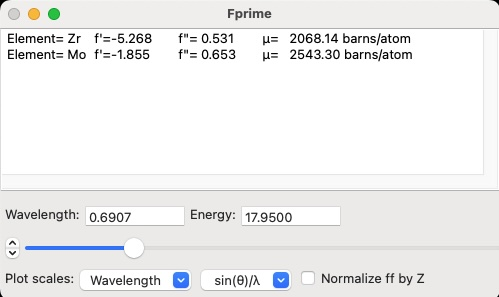
\includegraphics[width=0.5\linewidth]{figures/fprime3.jpg}
    \caption{Program Fprime: graphics window after shifting the wavelength near to an absorption edge. Note the change to the Zr $f^\prime$ value.}
    \label{fig:fprime3}
\end{figure}

\begin{figure}
    \centering
    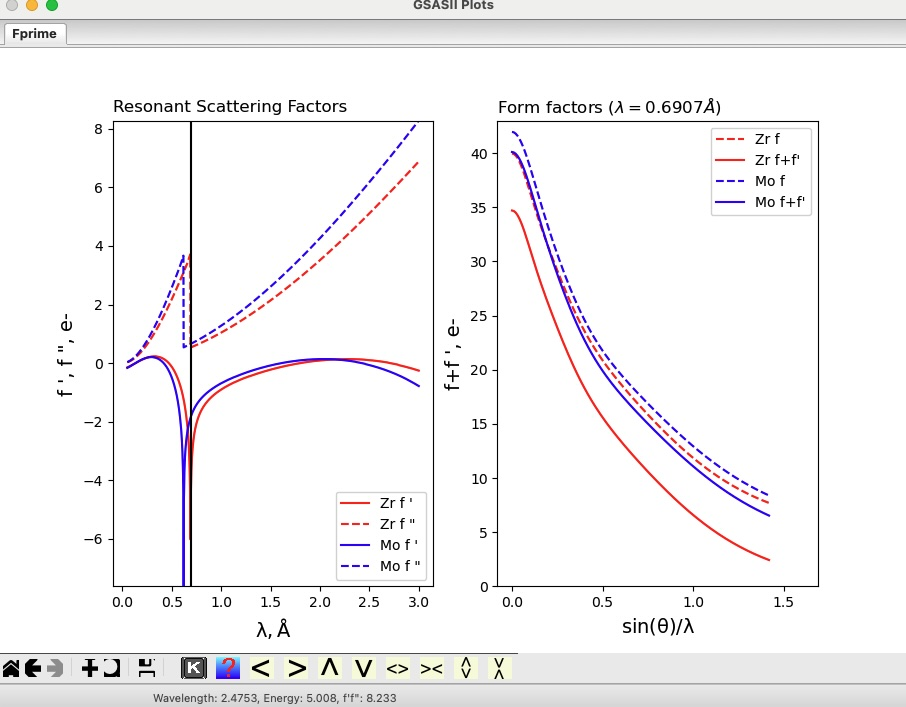
\includegraphics[width=1\linewidth]{figures/fprime4.jpg}
    \caption{Program Fprime: graphics window after shifting the wavelength near to an absorption edge. Note the change to the Zr scattering factor curve.}
    \label{fig:fprime4}
\end{figure}

To close the Fprime window, use the Fprime/Quit manu command. This will also close the tab on the plot window. 

\section{PlotXNFF: Plot form factors and scattering lengths}\label{ref:PlotXNFF}

The PlotXNFF program is supplied to plot the form factors for x-rays, neutrons, electrons and magnetic scattering for neutrons using the scattering factor tables supplied with GSAS-II. To access it, use the Calculate/"Run PlotXNFF" menu command. This will open an empty window. The next step is to select an element that will be used in the computation. Use the File/"Pick Element" menu command, which opens a periodic table. Click on an element in the table. That element is immediately selected and the plots are updated to show the scattering lengths and the form factors for the database contents. As an example, the element Ti is selected. The empty window remains empty, but a new plot window is opened and there are four plots available, of which three are shown in Figs. \ref{fig:XNFF1}, \ref{fig:XNFF2} and \ref{fig:XNFF3}.

\begin{figure}
    \centering
    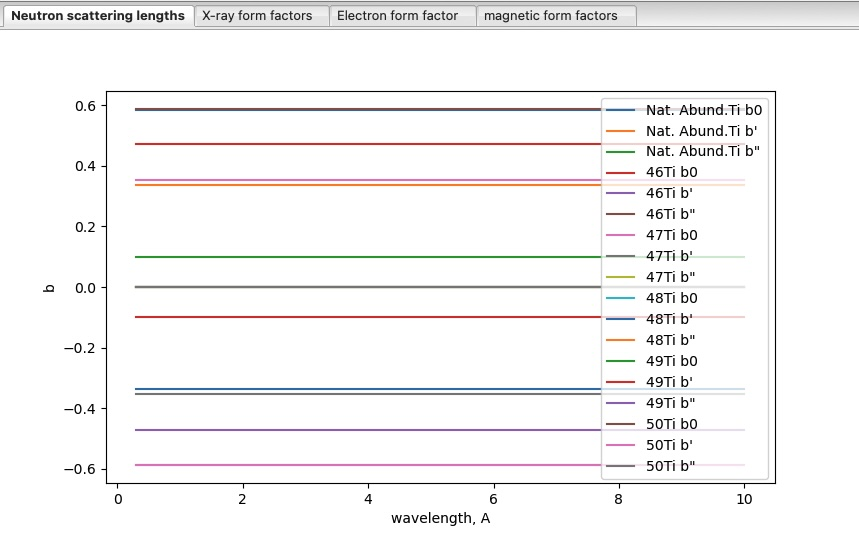
\includegraphics[width=0.8\linewidth]{figures/XNFF1.jpg}
    \caption{Program PlotXNFF: Neutron scattering lengths for Ti at natural abundance and for the isotopes of Ti listed in the GSAS-II database..}
    \label{fig:XNFF1}
\end{figure}

\begin{figure}
    \centering
    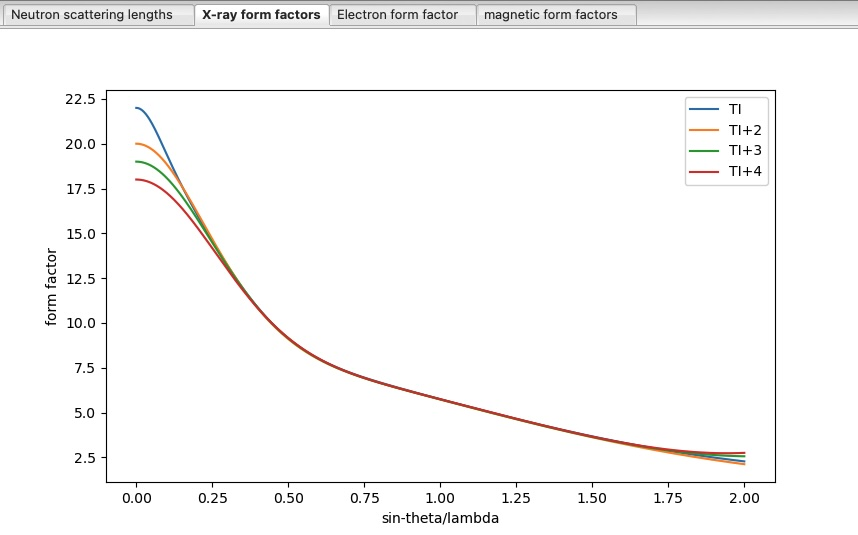
\includegraphics[width=0.8\linewidth]{figures/XNFF2.jpg}
    \caption{Program PlotXNFF: X-ray form factors for Ti several oxidation states. Note that the curves are nearly identical above $\sin\theta/\lambda$ of 0.2 \AA$^{-1}$ (Q >= 2.5 \AA$^{-1}$) .}
    \label{fig:XNFF2}
\end{figure}

\begin{figure}
    \centering
    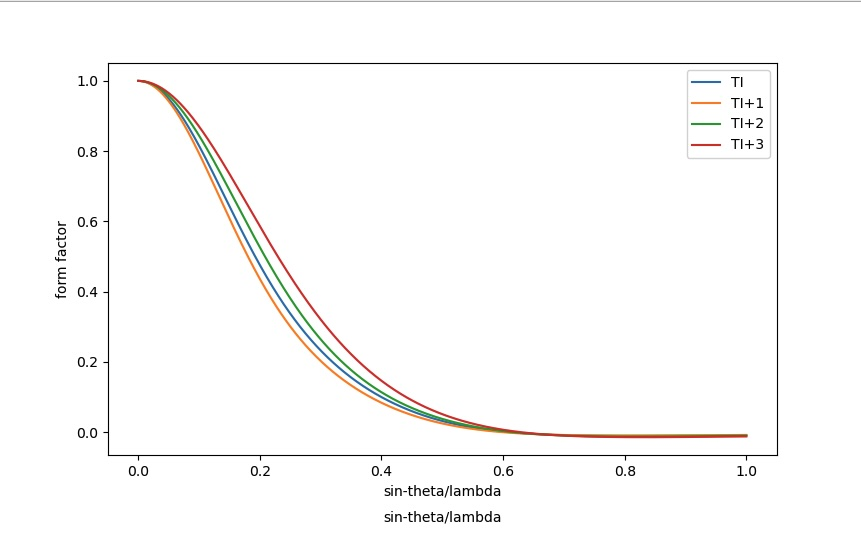
\includegraphics[width=0.8\linewidth]{figures/XNFF3.jpg}
    \caption{Program PlotXNFF: Neutron magnetic scattering for different oxidation states of Ti. Note that the scattering is close to zero above $\sin\theta/\lambda$ of 0.5 \AA$^{-1}$ (Q >= 6.3 \AA$^{-1}$) while in Fig. \ref{fig:XNFF2}, with the x-ray form factor the scattering power has dropped only by about 50\%.}
    \label{fig:XNFF3}
\end{figure}

Neutron form factors are usually independent of wavelength, but a few isotopes have neutron resonances, with an example shown in Fig. \ref{fig:XNFF4}. GSAS-II will attempt to compensate for the change in scattering length as a function of wavelength provided that the wavelength band used for time-focussing is narrow. If not, one is probably best discarding all neutrons collected at resonance wavelengths. In any case, knowing where the resonances occur is important for experiment planning. 

\begin{figure}
    \centering
    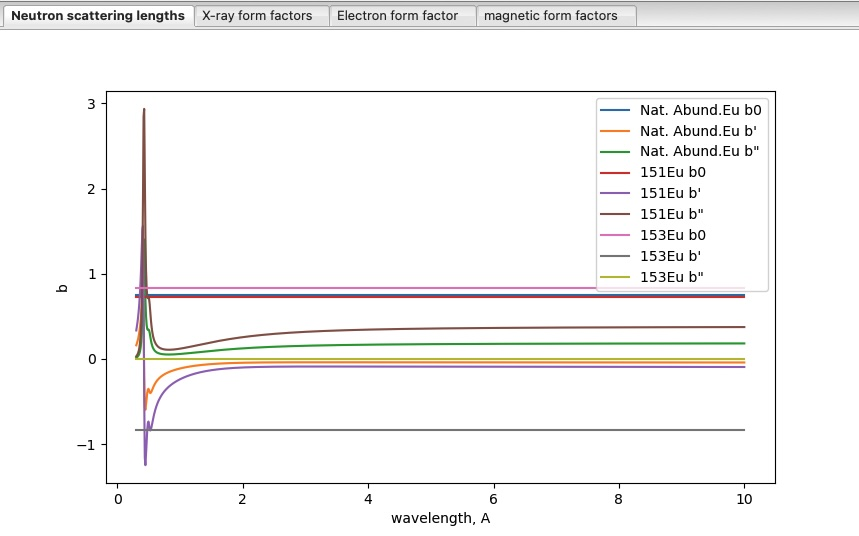
\includegraphics[width=0.8\linewidth]{figures/XNFF4.jpg}
    \caption{Program PlotXNFF: Neutron scattering lengths for Eu at natural abundance and for the isotopes of Eu listed in the GSAS-II database. Note that these isotopes have strong neutron resonances, which will change the scattering power significantly at shorter neutron wavelengths.}
    \label{fig:XNFF4}
\end{figure}